%%%%%%%%%%%%%%%%%%%%%%%%%%%%%%%%%%%%%%%%%%%%%%%%%%%%%%%%%%%%%%%%%%%%%%%%%%%%%%%%

\documentclass[12pt, a4paper, oneside]{book}

\input{/home/giatro/.config/user/giatro_packages.tex}

\input{/home/giatro/.config/user/giatro_macros.tex}

\title{Lista 2 - MAC0425 - Inteligência Artificial}
\date{\today}
\author{Lucas Paiolla Forastiere}

%%%%%%%%%%%%%%%%%%%%%%%%%%%%%%%%%%%%%%%%%%%%%%%%%%%%%%%%%%%%%%%%%%%%%%%%%%%%%%%%
%%%%%%%%%%%%%%%%%%%%%%%%%%%%%%%%%%%%%%%%%%%%%%%%%%%%%%%%%%%%%%%%%%%%%%%%%%%%%%%%

\begin{document}

\maketitle

\paragraph{1.}%
\label{par:1_}

Os experimentos foram feitos utlizando o arquivo \texttt{qlearn.py} (basta ter
\texttt{python} e a biblioteca \texttt{numpy} instalados e rodar utilizando
\texttt{\$ python qlearn.py}). Utilizando o programa, obtemos os seguintes
\textit{q-values} após 5 iterações:

\begin{figure}[h]
\centering
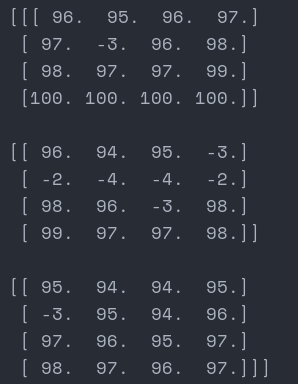
\includegraphics[scale=0.8]{Res/q-values-ex1.png}
\caption{O \texttt{ndarrary} dos \textit{q-values} para o exercício 1. Como cada
estado possui 4 ações, então temos um tensor de três dimensões. Para visualizar
esse tensor em duas dimensões (no terminal) }
\label{q-values-ex1.png}
\end{figure}

Na imagem





%%%%%%%%%%%%%%%%%%%%%%%%%%%%%%%%%%%%%%%%%%%%%%%%%%%%%%%%%%%%%%%%%%%%%%%%%%%%%%%%

\end{document}
